% Historical source (removed by author request): references/_OLD_Übungsaufgaben/Übungsblatt 3 - Vektorechnung/Blatt3.tex:270
\begin{ExerciseBlock}
\ExerciseHeading{11}{Satz von Thales}{vector_algebra_thales_theorem}
Der Satz von Thales besagt, dass die Vektoren $\vec{a}$ und $\vec{b}$, die jeweils die Randpunkte eines Halbkreises mit einem beliebigen Punkt auf dem Halbkreis verbinden, senkrecht aufeinander stehen. (siehe Abbildung) Dieser Satz soll nun bewiesen werden. 

\begin{center}
	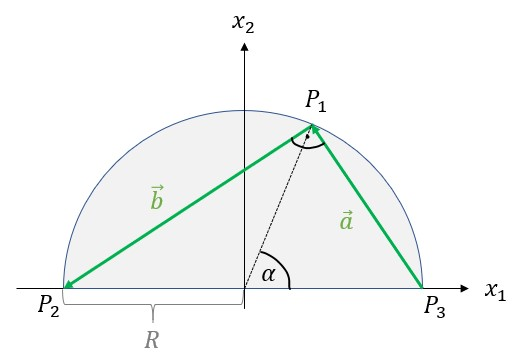
\includegraphics[width=0.55\textwidth]{content/resources/chapters/vector_algebra/images/thales_theorem.png} 
\end{center}

\begin{enumerate}[label=\alph*)]
	\item Geben Sie die Koordinaten der Punkte $P_1$, $P_2$ und $P_3$ an.
	\item Bestimmen Sie die Koordinatendarstellung der Vektoren $\vec{a}$ und $\vec{b}$.
	\item Zeigen Sie, dass die Vektoren $\vec{a}$ und $\vec{b}$ senkrecht aufeinander stehen.
\end{enumerate}

\end{ExerciseBlock}
\UseExerciseSolution{vector_algebra_thales_theorem}
